\documentclass{llncs}
\usepackage{llncsdoc}

\usepackage[english]{babel}
\usepackage[utf8]{inputenc}
\usepackage{amsmath}
\usepackage{graphicx}
\usepackage[colorinlistoftodos]{todonotes}
\usepackage{wrapfig}
\usepackage{makeidx}  % allows for indexgeneration
\usepackage{bibspacing}
\usepackage{fancyvrb}
\usepackage{amsfonts}
\usepackage{color}


\setlength{\bibspacing}{\baselineskip}
\usepackage[tight,footnotesize]{subfigure}
 

\newcommand{\mySection}[1]{\vspace{-5pt}\section{\hskip -1em.~~#1}\vspace{-10pt}}
\newcommand{\mySubSection}[1]{\vspace{-5pt}\subsection{\hskip -1em.~~#1}\vspace{-10pt}}
\newcommand{\mySubSubSection}[1]{\vspace{-5pt}\subsubsection{\hskip -1em.~~#1}\vspace{-5pt}}
\newcommand{\tableref}[1]{Table~\ref{tab:#1}}
\newcommand{\figref}[1]{Fig.~\ref{fig:#1}}
\newcommand{\Hao}[1]{$\clubsuit$\footnote{HAO: #1}}


\title{Domain-Knowledge-Guided Environment Model Abstraction and Refinement for Medical Device Software Verification}

%\author{You}

%\date{\today}

\begin{document}
\maketitle

\begin{abstract}
Implantable medical devices are designed to diagnose and improve certain adverse physiological conditions, thus the safety and efficacy of the devices have to be evaluated in closed-loop within their physiological context. Model-based design has enabled closed-loop verification early in the design stage and closed-loop model checking has been proposed to provide confidence in the safety and efficacy of the devices. One of the biggest challenge for model-checking is to balance the complexity and the expressiveness of the models. The Counter-Example-Guided Abstraction and Refinement (CEGAR) framework has been developed to reduce the complexity of the model using over-approximation and refine the model when false-positives are found. In system modeling, there is only one valid system, so that any behaviors in a system model that cannot be produced by the system are regarded as spurious. However in environment modeling, an environment model generally abstracts multiple environment conditions, therefore determining the validity of a closed-loop execution is not intuitive, making it difficult to apply CEGAR during environment modeling. On the other hand, the development of environment models and validation of closed-loop executions rely heavily on domain expertise. It is therefore possible to encode the domain knowledge during environment modeling and provide guidance during the refinement of the environment models. In this paper, we use implantable pacemaker as example to illustrate the challenges for applying CEGAR during environment modeling, and how to use encoded domain knowledge to guide the environment model abstraction and refinement.
\end{abstract}

\section{Introduction}
%\begin{itemize}
	%\item What are Cyber-Physical Systems?
    %\item What are the unique challenges of developing CPS compared to other systems?
    %\item How to guarantee the safety of CPS?
    %\item What is the current practice?
    %\item What is the difference between requirements and specifications?
    %\item What is closed-loop verification? Is it necessary?
    %\item What is model-based design? What are the benefits and limitations?
    %\item What are the different techniques of model-based closed-loop verification? 
    %\item In which steps during the software life cycle are those techniques used?
    %\item What is model checking? What guarantee can it provide? What are the challenges?
    %\item What are the focus difference between environment modeling and system modeling, in general and in each step?
    %\item What is model abstraction/approximation? What information are lost during this process?
    %\item How to keep track of these information? Where can they be used?
    %\item What is over-approximation? What are the limits?
    %\item What is the appropriate model complexity?
    %\item What aspects affect the required model complexity?
    %\item How to manage complexity for the system model?
    %\item Why CEGAR cannot be applied to the environment model?
    %\item How to manage the complexity of the environment model?
    %\item What are domain knowledge? Where have we used them?
    %\item How can we encode domain knowledge used during model development and abstraction?
    %\item Can we use encoded domain knowledge to manage complexity of the environment model? How?
    %\item The case study on heart model and pacemaker sounds good. Is the approach general enough?
%\end{itemize}

Implantable medical devices like pacemakers are designed to improve certain undesired physiological conditions with very little human interventions. Their capability of autonomously affecting the physiological conditions of the patients makes the medical devices safety-critical, and sufficient evidence on the safety and efficacy of the devices should be provided before the devices can be implanted in the patients. As more functions added to the devices, the complexity of the software component of the device is increasing dramatically, leading to more and more potential safety violations due to software bugs. To ensure the safety of medical device software, the device software not only have to conform with its design, which is specified in \emph{Software Specifications}
\subsection{The Model Checking Problem}
%Model-based design enables closed-loop verification at an early design stage. 
For a model $M$ with state space $S$, we define the behavior of the model as an execution trace in $\delta\in S^*$. The reachable behavior space of model $M$ is denoted as $\mathbb{B}(M)\subset S^*$. A property $\varphi$ defines a region in the behavior space within which the property is satisfied, which can be denoted as $\mathbb{B}(\varphi)$. A model checking problem is to use mathematical tool to explore the whole reachable behaviors of a model $M$ against a property $\varphi$ such that $\mathbb{B}(M)\subseteq \mathbb{B}(\varphi)$. We denote it as $M\models\varphi$. Property violations should be returned as execution traces $\delta_v$ so that the designer can analyze and address the problem. 

\subsection{Model Abstraction with Over-approximation}
The behavior space of the actual system is too large for model checker to exhaustively explore. A model of the system which covers all behaviors of the system can be developed which can not only reduce complexity, but also having the suitable formalism for the model checker. An abstraction function $h$ abstracting model $M$ to $M'$ is a non-surjective function from state space $S$ to the new abstract state space $S'$ such that: 
$$\forall s\in S, \exists s'\in S' \text{ s.t. } h(s)=s'$$
This definition can be extended to behaviors $\delta\in \mathbb{B}(M)$, such that:
$$\forall \delta\in \mathbb{B}(M),\exists \delta'\in\mathbb{B}(M')\text{ s.t. } h(\delta)=h(\delta')$$
From the definition, we know that the abstract model $M'$ covers all behaviors of $M$, which is referred to as \emph{over-approximation}. We represent the over-approximation relationship as $M'\models M$, and the relationship between reachable behavior spaces as $\mathbb{B}(M)\subset_a\mathbb{B}(M')$. Then we have:
$$\mathbb{B}(M')\subseteq_a \mathbb{B}(M),\mathbb{B}(M)\subseteq_a \mathbb{B}(\varphi)\rightarrow\mathbb{B}(M')\subseteq_a \mathbb{B}(\varphi)\rightarrow M_t\models\varphi$$
Since the properties are preserved In general the state space of $S'$ is smaller than $S$ while still preserve the property, during model checking the more abstract model can be used to check the property. 

\subsubsection{Context Ambiguities}
Since $h$ is non-surjective, certain states in $S$ will not be distinguishable in $S'$:
$$\exists s_1,s_2\in S \text{ s.t. }h(s_1)=h(s_2)=s',s'\in S'$$
For behaviors we have:
$$\exists \delta_1,\delta_2\in \mathbb{B}(M) \text{ s.t. }h(\delta_1)=h(\delta_2)=\delta',\delta'\in \mathbb{B}(M')$$
In the abstract model $\delta_1$ and $\delta_2$ are not distinguishable
\subsubsection{Validity Ambiguities}
However since $h$ is non-surjective, there exists behaviors in $M'$ that do not exists in the original model $M$:
$$\exists\delta'\in\mathbb{B}(M')\text{ s.t. }h^{-1}(\delta')\not\subset\mathbb{B}(M)$$

\subsubsection{System Model vs. Environment Model}
\subsection{Closed-loop Model Checking}
%During the software development process, there are two key documents that track the safety and efficacy of the software component, namely the \textbf{Software Requirements} and \textbf{Software Specifications}. These two terms are sometimes used interchangeably, however, requirements and specifications provides different angle of system safety and require very different verification techniques.
%
%A requirement states the objective of the system in design in terms of environmental conditions. For example, a requirement of a self-driving car would be: \emph{The car should not hit a pedestrian.} A specification is how the system developers propose to satisfy the requirements. For example, the specification corresponding to the requirement of a self-driving car would be: \emph{If an object is detected in front of the car and the distance to the object is less than $d$, the car should brake.} As we can see, a specification may not satisfy the corresponding requirement, thus two steps are required to guarantee the safety of the system software. The first is the conformance between the system software and the software specification. The second one is whether the software specifications can satisfy all the software requirements.
%
%Currently in most system design, the conformance between the software specifications and the system software are verified using extensive \textbf{open-loop} testing. The test cases are extracted from the system software using static analysis based on certain coverage criteria. The conformance between the specifications and the requirements are maintained by traceability documents, which is insufficient for safety guarantee.
% \begin{figure}[!t]
% 		\centering
% 		\includegraphics[width=0.8\textwidth]{figs/SysVSEnv.png}
% 		%\vspace{-5pt}
% 		\caption{\small Modeling in terms of behavior coverage. As model becomes more abstract, the coverage increases while the boundary becomes more simple. (a) System modeling in which there is only one concrete system; (b) Environment modeling in which abstraction can be used to generalize different conditions}
% 		  %\vspace{-15pt}
% 		\label{fig:sys}
% \end{figure}
\begin{figure}[!t]
		\centering
		\includegraphics[width=0.8\textwidth]{figs/distinction.png}
		%\vspace{-5pt}
		\caption{\small }
		  %\vspace{-15pt}
		\label{fig:ambiguity}
\end{figure}
\begin{figure}[!t]
		\centering
		\includegraphics[width=0.8\textwidth]{figs/env_sys.png}
		%\vspace{-5pt}
		\caption{\small }
		  %\vspace{-15pt}
		\label{fig:distinction}
\end{figure}

Since the requirements describe the intended behaviors of the closed-loop system consists of the environment and the system, verifying whether the specifications of the system satisfy the requirements requires closed-loop verification. In the medical device industry, closed-loop verification is performed in the form of clinical trials in which the devices are tested on the real patients. Clinical trials can only cover very limited environmental conditions due to extremely high cost. Moreover, clinical trials are often conducted at the last design stage. Fixing bugs at this stage is also very costly.

Model-based design has been proposed to speed up system software design and provide sufficient safety maintaining the safety promises in software requirement. It can potentially enable closed-loop verification of the software requirements at an earlier stage thus reduce cost. In a model-based design framework, the system software is first designed as an abstract model. Together with an environment model the closed-loop system can be verified against software requirements using model-checking techniques. The verified system model can then be rigorously translated into the software implementation (semi-)automatically so that the software implementation also satisfies all the software requirements.

%The software and its environment have very different properties that modeling them requires very different focuses. The software is generally a control graph which is generally deterministic given with physics and computations are two different things.

One of the biggest challenge for model-based design is to manage how much detail a model should have during model checking. In general the model should be abstract enough to ignore unnecessary details in order to reduce computational cost, but also detailed enough to distinguish execution paths that 1) satisfy/violate a property, and/or 2) are valid/invalid due to the extra behaviors introduced during model abstraction/approximation. These ambiguities must be removed from model to prevent false positives/negatives during model checking. 

\subsection{Outline of the paper}
\begin{itemize}
	\item Section 2: Basic state space formulation with transition groups
    \item Section 3: Formulation of over-approximation and its effect on transition groups
    \item Section 4: Linking transition groups to environmental conditions and thus requirement
    \item Section 5: Rule-based EP heart model abstraction with transition groups
    \item Section 6: Case 1: Requirement-guided model refinement during ELT case 
    \item\textcolor{red}{ Section 7: Case 2: Model refinement for eliminating potential ambiguity. With mode-switch case.} 
\end{itemize}

%\section{Closed-loop Model Checking}
%We first define the behavior space of a model as all combinations of states valuations. For a model $M$ with $n$ state variables $v_1\dots v_n$, and each state variable can take value within the domain $D(v_i)$, the size of the overall behavior space is $\Pi_{i=1}^n D(v_i)$. The actual reachable behavior space of a model $M$ is far less and can be defined by $\mathbb{B}(M)$. As a reference or ground truth for behavior space, we assume the behavior space $\mathbb{B}(S)$ for a physical system $S$ which is infinitely large. All the behavior spaces correspond to the models $\mathbb{B}(M)$ of the system are projections from $\mathbb{B}(S)$.  
%\Hao{}
For a model $M$ with state space $S$, we define the behavior of the system as an execution trace in $\delta\in S^*$. The reachable behavior space of model $M$ is denoted as $\mathbb{B}(M)\subset S^*$.

An abstraction function $h$ is a surjection from

No models of the system can match the region of the system exactly due to lack of information. As the model becomes more abstract, the boundary defining the behavior region becomes less complex. If the abstract model covers all the system behaviors such that $\mathbb{B}(S)\subset\mathbb{B}(M)$, the model is referred to as an \emph{over-approximation} of the system. For environment model, over-approximation can also be used to \emph{generalize} different environmental conditions, i.e. in \figref{distinction}.(a) two system behaviors $\mathbb{B}(S_1)$ and $\mathbb{B}(S_2)$ are covered by a model $\mathbb{B}(M)$.

A property defines a region in the behavior space within which the property is satisfied. The satisfaction region of a property $\varphi$ can be denoted as $\mathbb{B}(\varphi)$. 
A system $S$ satisfies a property $\varphi$ if $\mathbb{B}(S)\subseteq \mathbb{B}(\varphi)$. We denote it as $S\models\varphi$. As we can see, if $M$ is an over-approximation of $S$, meaning $\mathbb{B}(S)\subseteq \mathbb{B}(M)$, and $\mathbb{B}(M)\subseteq \mathbb{B}(\varphi)$, we have $\mathbb{B}(S)\subseteq \mathbb{B}(\varphi)$, meaning $S\models\varphi$. 

In most of the cases, the internal states and transitions of a system cannot be fully observable. The behavior space can thus be mapped to other observable behavior spaces with less dimensions.
\Hao{Need to clarify/visualize the notion of observability here} 
Note that the observability does not refer to the interface of the system, there can be multiple observable behavior spaces that correspond to different abstraction of the system. As the result, behaviors that are distinguishable in the full behavior space can be indistinguishable in a observable behavior space, causing ambiguities that can result in false-negatives and false-positives during verification. We denote one observable behavior space as $\mathbb{B}_o(S)$. 

As shown in \figref{distinction}, $\mathbb{B}(M)$ and $\mathbb{B}(\varphi)$ are mapped to $\mathbb{B}_o(M')$ and $\mathbb{B}_o(\varphi')$. Three behaviors in $b_1,b_2,b_3\in\mathbb{B}$ are mapped to a single behavior $b'\in\mathbb{B}_o$. Since $b'\not\in\mathbb{B}_o(\varphi')$, it may be returned by verification tools like model checker as counter-example. In $\mathbb{B}_o$ is possible that two categories of ambiguities exist, namely \textbf{Validity ambiguity} and \textbf{Context ambiguity}. %Failure to distinguish these behaviors can cause false-negatives and/or false-positives during verification.

Validity ambiguity refers to the incapability to distinguish a physically possible execution with an invalid one. In \figref{distinction}.(a), $b_3$ is an invalid behavior since it does not belong to either $S_1$ or $S_2$ but it is covered by the model $M$. 

A model $M$ is compatible with an observable behavior space $\mathbb{S}^o$ if all the behaviors that can be generated by $M$ 

A model is appropriate for a property if all its behaviors  



A Counter-Example-Guided Abstraction and Refinement approach has been proposed to automatically derive model with appropriate amount of details. (\cite{CEGAR}) Assume we would like to check the system $S$ against the property $\varphi$. First, the most abstract model $M_0\models^a S$ is derived from the actual system $S$ based on certain abstraction rules, so that it can distinguish all execution paths that satisfy/violate $\varphi$. Then $M_0$ is verified against the property in an automated model checker. If the property is violated $M_0\not\models\varphi$, a counter-example $\delta^c$ is returned by the model checker. $\delta^c$ has to be then validated so that it can be produced by $S$. If the system can produce $\delta^c$, which can be denoted as $\delta^c\triangleleft S$, $\delta^c$ is a valid counter-example. Otherwise $\delta^c$ is regarded as \textbf{spurious} and the model has to be refined so that the $\delta^c$ is not producible by the model. The refined model $M_1\models^a M_0$ is derived by adding back the minimum amount of abstracted details that prevent $\delta^c$ from being enabled, so that $\delta^c\not\triangleleft M_1$. This process continues until either no counter-example is returned, or a counter-example is not spurious. 

CEGAR works very well during system modeling in which there is only one concrete system implementation $S$. However, for closed-loop verification the objective is to check whether $E||S\models\varphi$. If the environment $E$ is also represented by a model during model checking, both $M^E$ and $M^S$ have to be unambiguous. When verifying system specifications, normally there is no constraints on the environment so that there is no spurious counter-examples due to the environment model. In this case CEGAR still works. However in the software requirements, there are constraints on the environment conditions. If these constraints are not enforced in $M^E$, the verification can yield spurious counter-examples. However, CEGAR will not work for environment modeling due to the differences between the environment and the system. In system modeling, there is only one concrete implementation $S$, so if a counter-example $\delta^c$ is returned during model checking, only $\delta^c\triangleleft S$ has to be checked. However, for the environment, there are infinite number of environmental conditions $E_i$, like different patients in the medical device domain. Details are ignored in the abstract models not only to reduce complexity, but also to \textbf{generalize} different conditions so that:
$$\forall \delta\triangleleft E_i, i\in [1,n],\delta\triangleleft M^E$$
Note that during the generalization process, more behaviors of the environment will be introduced into the model: 
$$\exists\delta^s\triangleleft M^E \text{ s.t. } \delta^s\not\triangleleft E_i, i\in [1,n]$$
In this case, if an execution path $\delta$ is returned as a counter-example during model checking on software requirement, there is no way to check whether 
$$\exists i\in[1,n],\delta\triangleleft E_i$$ 
as $n$ may be a large number or is unclear in the first place. As a result, the validity of the counter-example cannot be validated, and therefore the model cannot be refined by analyzing the spurious counter-example. CEGAR is not effective during environment modeling.

In Cyber-Physical Systems, there are \textbf{domain experts} who understand how the environment of the system works. The \textbf{domain knowledge} is a set of environmental constraints which can be used to define different environment conditions, and determine the validity of the execution paths. However, domain knowledge are in general not formalized thus cannot be used in any automated processes. In this paper, we use closed-loop model checking on an implantable pacemaker model as example to demonstrate abstraction and refinement of the environment models using encoding domain knowledge. We use two case studies to demonstrate that although CEGAR is not applicable to the environment model, the domain knowledge can still be used to validate executions and provide potential validity violations.\Hao{Still need to formalize}

The contribution of this paper is two-folds: 1) we formally specified the potential ambiguities during model abstraction and identified the difference between environment modeling and system modeling. 2) We demonstrated the potential application of encoded domain knowledge to eliminate the ambiguities during abstraction and refinement of environment models.
\begin{itemize}
	\item Abstraction rules for environment models 
    \item Appropriate abstraction function check, definition clear, assumptions implicit, especially for environment models
\end{itemize}
%\section{A Simple Example}
Imaging we are developing a high-level control algorithm for an autonomous vehicle
\textsf{A[] (not CarCross $\&\&$ PedCross)}\\
\textsf{E<> (CarCross)}
\begin{figure}[!t]
		\centering
		\includegraphics[width=0.9\textwidth]{figs/example.png}
		%\vspace{-5pt}
		\caption{\small }
		  %\vspace{-15pt}
		\label{fig:example}
\end{figure}

\section{State Space Formulation}
Kripke structure $<S,\Sigma,L,I>$ in which $S$ is a set of states, $\sigma(s_1,s_2)\in\Sigma\subset S^2$ is a set of transitions, $I\subset S$ is a non-empty set of initial states.

To clarify things, we first introduce \emph{state groups} and \emph{transition groups}. The state space is defined by state variables. 
$$s\{\theta_1,\theta_2\dots \theta_n\}\in S$$
Each state $s$ is a valuation of all the state variables. Partial valuations can be used to represent a state group. For example, $s\{\theta_1=v_1\}$ represents all states in which $\theta_1=v_1$.

Each state transition $\sigma\in\Sigma$ is defined as $\sigma(s_1,s_2)$ such that:
$$s_1\xrightarrow{\sigma}s_2\text{ in which }s_1,s_2\in S$$
Certain transitions have the same behaviors, mostly observablly equivalent . It is convinient to group them together to describe the behaviors of the system. A \textsf{transition group} is a group of transitions that the pre- and post- states satisfy certain criteria:
$$\Sigma_\phi\subset\Sigma \text{ s.t. }\forall\sigma(s_1,s_2)\in\Sigma_\phi,f(s_1,s_2)\models\phi,s_1,s_2\in S$$
in which $f(s_1,s_2)$ is certain proposition of the two states or their substates. It is possible that $\Sigma_{\phi_1}\cap\Sigma_{\phi_2}\neq \emptyset$.

Ideal execution path of length n: $\delta:s_0\sigma_0\dots\sigma_i\dots\sigma_ns_n\in\Sigma^*$ in which: 
$$s_0\in I, \sigma_i(s_i,s_{i+1})\in\Sigma, i\in[0,n-1]$$ 
The set of all the transitions in a path is represented by $\Sigma_\delta$.

Each transition takes time. We denote it as $t=T(\sigma)$. The time for each execution path: $$T(\delta)=\sum_{i=0}^nT(\sigma_i)$$

Partial paths: Not all the transitions in a path are necessary. In fact, ideal paths are not possible, so do ideal models. One way to represent partial paths is timed execution path: sequence of transitions with unobservable ones abstracted with time lapse $\delta_t\in(\sigma_o,t)^*, t\in \mathbb{R}$

$\delta_t$ is an abstraction of $\delta$, we denote it as $\delta\models\delta_t$. For a execution path 
$$\delta=\sigma_0\sigma_1\dots\sigma_n$$
there is a corresponding timed execution path 
$$\delta^t=(\sigma_0^t,t_0)(\sigma_1^t,t_1)\dots(\sigma_m^t,t_m)$$ 
in which
$$\forall i,j,k \text{ s.t. } \sigma_i=\sigma_k^t,\sigma_j=\sigma_{k+1}^t,(\sigma_{i+1}\dots\sigma_{j-1})\neq\sigma_{j},T(\sigma_i\dots\sigma_j)=t_{k+1}-t_k$$
with length $m<n$ such that $\delta\triangleleft\delta^t$. 

Execution path produceable by model
$$\delta\in^p M$$
\subsection{A1: Observability Distinction}
The lowest distinction requirement for a model

The most basic observable transitions are input and output of the entity under modeling

Input triggered transitions $\Sigma_i$

Output inducing transitions $\Sigma_o$

If we have a timed trace such that $\delta\triangleleft\delta_t$, all the transitions in a path $\delta$ which are input/output transitions should be preserved in the timed trace $\delta_t$. 
%$$\delta\triangleleft\delta^t\rightarrow\forall \sigma\in(\Sigma_i\cup\Sigma_o)\cap\Sigma_\delta,\sigma\in\Sigma_(\delta_t)$$

A model $M$ is observability distinctive iff
$$\forall\delta^t\in^p M, \forall\delta\triangleleft\delta^t,\forall \sigma\in(\Sigma_i\cup\Sigma_o)\cap\Sigma_\delta,\sigma\in\Sigma_{\delta^t}$$
The observability of the system and the environment are different. After the system has been developed, the observability of the environment is fixed. However, for the system itself, the observability can range from full white-box (code level) to full blackbox (input-output only)

\subsection{A2: Property Distinction}
We refer a model $M$ is property distinctive for property $\phi$ by $M\triangle\phi$, such that

$$\forall \delta^t\in^p M, \delta^t\models\phi\leftrightarrow\forall \delta\triangleleft\delta^t,  \delta\models\phi$$
%$$\forall \delta_1,\delta_2\triangleleft\delta_t, \delta_1\models\phi\leftrightarrow \delta_2\models\phi$$

\subsection{A3: Validity Distinction}


For system model $M^s$
$$\delta^t\in^p M^s \text{ iff }\exists\delta\triangleleft\delta^t\text{ s.t. } \delta\in^p M^s$$


There can be multiple execution path correspond to the same timed execution path. 
$$\exists \delta_1,\delta_2\text{ s.t. } \delta_1\models\delta_t,\delta_2\models\delta_t$$
In this case, we say that $\delta_1$ and $\delta_2$ are not \textbf{distinguishiable}. 

Distinguishible transitions: a lot of the times two paths have to be distinguishible (healthy vs. unhealthy)


Trace produceable by model: For an execution path $\delta$ with length $n$, we denote that the path is produceable by model $M$ with $\delta\triangleleft M$, such that:
$$\forall \sigma(s_i,s_{i+1})\in \delta,i\in[0,n-1], s_0\in I, \sigma(s_i,s_{i+1})\in\Sigma_M$$

Timed trace produceable by model:


non-determinism

For system:
$$\delta\models\delta_t,\delta_t\triangleleft M_s \text {  iff  } \delta\triangleleft M_s$$
For environment:
$$\delta$$
%\section{Model Abstraction With Over-approximation}
%For two models $M_1$ and $M_2$, we denote $M_2$ is an abstraction of $M_1$ as $M_1\preceq M_2$. A function $s'=h(s),s\in S_1,s'\in S_2$ is a mapping from the states in $M_1$ to states in $M_2$. 
%
%For two models $M_1$ and $M_2$ such that $M_1\preceq M_2$, we know that all the transitions are preserved:
%$$\forall \sigma(s,s') \in\Sigma_1\text{ s.t. }s,s'\in S_1,\rightarrow\sigma(h(s),h(s')) \in\Sigma_2,h(s),h(s')\in S_2$$
%Due to the mapping the transition groups in $M_2$ are changed as well. For a transition group in $M_1$:
%$$\Sigma_{\phi1}\subset\Sigma_1 \text{ s.t. }\forall\sigma(s_1,s_2)\in\Sigma_{\phi1},f(s_1,s_2)\models\phi1,s_1,s_2\in E_1$$
%In the more abstract model, the propsition is often relaxed. For certain $\phi2\supseteq\phi1$, we have:
%$$\Sigma_{\phi2}\subset\Sigma_2 \text{ s.t. }\forall\sigma(h(s_1),h(s_2))\in\Sigma_{\phi2},f(h(s_1),h(s_2))\models\phi2,s_1,s_2\in S_1$$
%
%
%Some of the transition groups are merged. For two transition groups $\Sigma_{\phi1},\Sigma_{\phi2}\subset\Sigma_1$ there exists a new relation $\Sigma_{\phi3}\subseteq\Sigma_2$ such that: $$\phi1\cup\phi2\subseteq\phi3$$
%We denote this abstraction as:
%$$\Sigma_{\phi3}=\{\Sigma_{\phi1},\Sigma_{\phi2}\}$$
%We use $\Sigma_{\phi1}\lhd\Sigma_{\phi3}$ to represent the abstraction relationship between transition groups.
%\begin{itemize}
	%\item Over-approximation and its information loss
    %\item Abstraction in terms of transition groups
    %
%\begin{itemize}
	%\item Merging
    %\item \textcolor{red}{Remove}
%\end{itemize}
	%\item Assumptions made to simplify the model and increase model behaviors
    %\item Necessity of model refinements due to information loss
%\end{itemize}
%
%\subsection{System model vs. Environment model}
%\begin{itemize}
	%\item System model achieves simplicity during abstraction
    %\item Environment model also use abstraction to achieve generalization
    %\item Validation of counter-example cannot be done on a generalized environment model
%\end{itemize}

\section{\textcolor{red}{Requirement Encoding}}
\begin{itemize}
	\item Differentiate requirements from specifications.
    \item Requirements are environmental behaviors that the system want to achieve.
    \item It countains a pre-condition and post-condition, which can be linked to transition groups.
    \item 
\end{itemize}



\section{Rule-based Heart Model Abstraction}
\begin{figure}[!t]
		\centering
		\includegraphics[width=0.8\textwidth]{figs/rule.png}
		%\vspace{-5pt}
		\caption{\small Heart Model Abstractions}
		  %\vspace{-15pt}
		\label{fig:abs}
\end{figure}
Unlike system modeling in which there is only one concrete system, during environment modeling there are infinite number of environmental conditions that can be generalize by abstractions. In this section, we model the heart as the physiological environment for implantable pacemakers and try to cover different heart conditions and the closed-loop interactions between the heart and the pacemaker. Then using abstraction rules defined over physiological knowledge and principles for over-approximation we construct a series of heart model abstractions with different complexity and coverage. During the rule applications the merging of transition groups are documented thus can be used during model refinements.
\subsection{Electro-physiology (EP) Basics}
The heart generates periodic electrical impulses to control heart rates according to physiological needs. These impulses conduct through the heart, triggering coordinated muscle contractions and pump blood to the rest of the body. The underlying pattern and timing of these impulses determine the heart's rhythm and are the key to proper heart functions. Derangements in this rhythm are referred to as \emph{arrhythmia}, which impair the heart's ability to pump blood and compromise the patients' health. Arrhythmia are categorized into so-called \textsf{Tachycardia} and \textsf{Bradycardia}. Tachycardia features undesirable fast heart rate which results in inefficient blood pumping. Bradycardia features slow heart rate which results in insufficient blood supply. The electrical activities can be measured by inserting electrodes through the vein into the heart against the heart wall. Localized electrical activities can be measured, and the physicians can diagnose the heart conditions by delivering pacing sequence through the electrodes and observe the signal propagation. This procedure is referred to as Electrophysiological (EP) Testing  (\cite{josephson}) and the signals are referred to as electrograms (EGMs).

The implantable cardiac pacemakers are rhythm management devices designed to treat bradycardia. A typical dual chamber pacemaker has two leads inserted into the heart through the veins which can measure the local electrical activities of the right atrium and right ventricle, respectively. According to the timing between sensed impulses the pacemaker can deliver electrical pacing to the corresponding chamber to maintain proper heart rhythm.
\begin{figure}[!t]
\centering
		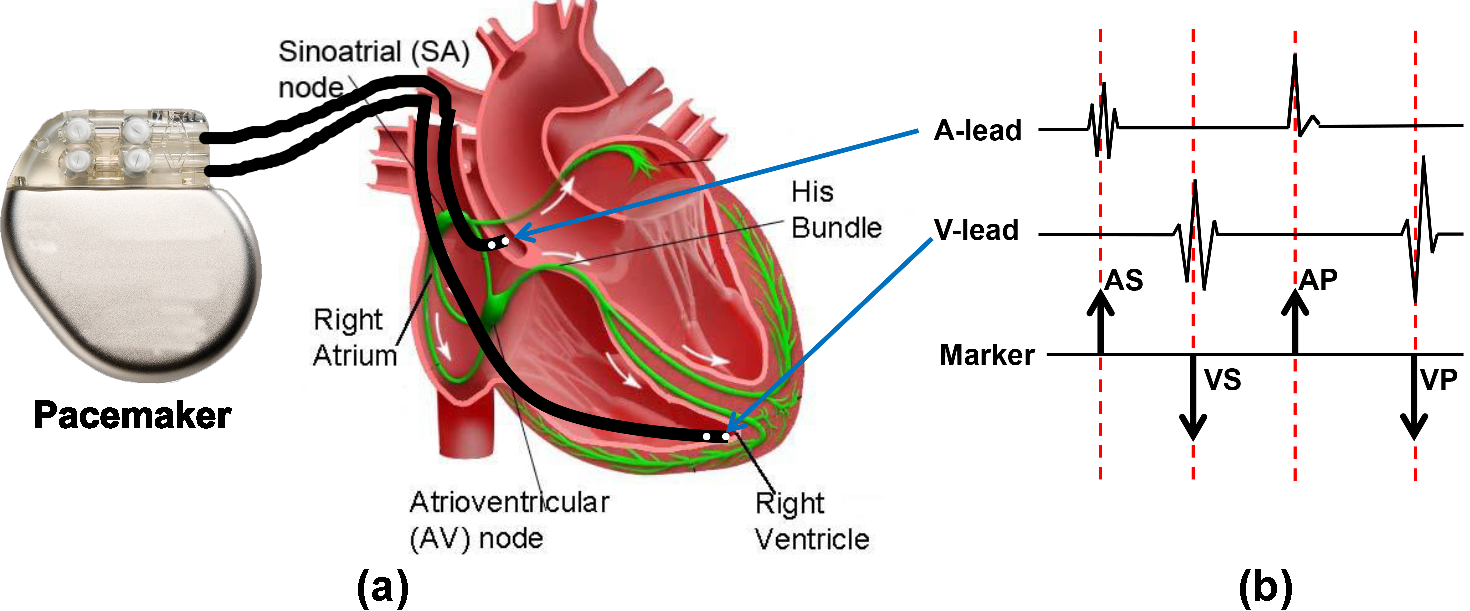
\includegraphics[width=0.7\textwidth]{figs/egm.pdf}
		
%\vspace{-10pt}
\caption{\small }
\label{fig:probes}
%\vspace{-15pt}
\end{figure} 
\subsection{The Initial Models}
In \cite{VHM_proc} we developed a heart model structure based on ElectroPhysiology (EP). We use an extended timed-automata formulation (\cite{timed_automata}) to model the timing behaviors of a heart tissue during each cycle. We refer the tissue model as \emph{Node automaton} and \figref{node_automata} shows the structure of a node automaton $i$. 3 states correspond to 3 timing periods of the action potential. From \textsf{Rest} state, the node can either self activate or activated by external stimuli (Act\_node) and go to \textsf{ERP} state. During \textsf{ERP} state the node does not respond to external stimuli (blocked). During \textsf{RRP} state, the node can still be activated and go to \textsf{ERP} state, however the ERP period and the conduction delay of the tissue are affected by the "earliness" of the activation arrived during the RRP period, which is tracked by a shared variable $C(i)$. The new ERP period is determined by a function over clock value $g(f(t))$ which mimic the beat-to-beat dynamics described in \cite{josephson}. 

The electrical conduction through the tissue between nodes are abstracted using \emph{path automata}. The path automata can be used to represent structural or topological (functional) electrical connections between nodes. \figref{path_automata} shows a path automaton connecting node a and b. The initial state of a path automaton is \emph{Idle}, which corresponds to no conduction. The states corresponding to the two conduction directions are named after the physiological terms: Antegrade (Ante) and Retrograde (Retro). These states can be intuitively described as forward and backward conductions. If \emph{Act\_path} event is received from one of the nodes connected to it, the a transition to \emph{Ante} or \emph{Retro} state correspondingly will occur in the path automaton. At the same time the clock invariant of the state is modified according to the shared variable \emph{C(a/b)}. This corresponds to the change of the conduction delay that is caused by the early activation. Similar to node automaton, the changing trend is extracted from clinical data. 
  \begin{figure*}[!t]
\centering
		\subfigure [\small]{			
		\includegraphics[width=0.35\textwidth]{figs/node_aut.png}
		\label{fig:node_automata}
		} 
%	\hspace{.1in}%
		\subfigure [\small] 
		{
		\includegraphics[width=0.35\textwidth]{figs/path_aut.png}
		\label{fig:path_automata}
		} 
		\subfigure [\small] 
		{
		\includegraphics[width=0.2\textwidth]{figs/gen_setup.png}
		\label{fig:general_setup}
		} 
\label{fig:h_automatas}
%\vspace{-10pt}
\caption{\small (a) Node automaton. Dotted transition is only valid for pacemaker tissue like SA node; (b) Path automaton; (c) Model of the electrical conduction system of the heart using a network of node \& path automata ~\cite{VHM_proc}.}
%\vspace{-15pt}
\end{figure*} 

\subsection{Rule 1: Remove nodes without self-activation and short ERP}
\begin{itemize}                                                                                                                                                                                                                             
	\item \textcolor{red}{Formal description}
    \item \textcolor{red}{Physiological justification}
    \item $H_0\rightarrow H_1$
    \item Transition groups merging during the abstraction
\end{itemize}

\subsection{Rule 2: Merge nodes with self-activation}
Three nodes and two paths. $H_1\rightarrow H_2$
\subsection{Rule 3: Replace ERP with non-deterministic conduction}
Two nodes and one path. $H_2\rightarrow H_3$
\subsection{Rule 4: Replace conduction with self-activation}
Two nodes. $H_3\rightarrow H_4$

\section{Case 1: Resolving Context Ambiguities Using Model Refinement}
\subsection{Endless-loop Tachycardia}
\subsection{\textcolor{red}{Requirement Encoding}}
\begin{itemize}
	\item Pre-condition: Regular atrial rate, possible ventricular tachycardia
    \item Post-condition: Ventricular pace rate no faster than max(atrial rate, LRI)
    \item $\sigma_{n1a}$ in pre-condition
\end{itemize}
\subsection{Why CEGAR does not work?}
\begin{itemize}
	\item Potential counter-example trace if $H_4$ is used
    \item Different concrete traces that the counter-example can correspond to
    
    \begin{itemize}
    	\item Valid and harmful
        \item Valid and unharmful
        \item Invalid
    \end{itemize}
\end{itemize}
\subsection{Requirement-guided model refinement}
\begin{itemize}
	\item The most abstract model with no ambiguities
    \item $\sigma_{n1a}$ is in $H_3$.
    \item Environment model refined to $H_3$
    \item Counter-example corresponds to real bug
\end{itemize}

\section{\textcolor{red}{Case 2: Resolving Validity Ambiguities Using Model Refinement}}
\subsection{Atrial Tachycardia and Mode-switch}
\subsection{Requirement Encoding}
\begin{itemize}
	\item Pre-condition: Atrial Tachycardia, vent  ricular rate normal
    \item Post-condition: No increase in ventricular rate
\end{itemize}
\subsection{Identify potential ambiguities}

\begin{itemize}
	\item Utilizing the assumptions made during abstraction Rule 3
    \item Replacing ERP with non-deterministic conduction can potentially increase the number of activations
    \item Two possible refined executions
    
\begin{itemize}
	\item Valid 
    \item Invalid
\end{itemize}
    \item Undo Rule 3
    \item Refine to $H_2$
\end{itemize}
\newpage
\section{Bullet Points}
\subsection{Specification vs. Requirement}
\begin{itemize}
	\item Requirements are specified in terms of conditions of the \textbf{environment} before and after the system is deployed
    \item Specifications are specified in terms of how the system responds to an input sequence from the environment
    \item Traditional verification focus on specification of the system
    \item Verifying specification only need to consider the input-output sequence of the system, which does not require knowledge of the environment
    \item The result only provide guarantees for the correctness of the system. But what about the correctness of the specifications themselves?
   
    \item In CPS especially, the focus should be more on whether specifications satisfy requirements, which is also an important aspect in requirement engineering.
    
    \begin{itemize}
        
        \item Requirements are specified by domain experts and requires deep domain knowledge 
        \item Traceability between requirements and specifications are currently maintained by mostly documentation
        \item Verifying requirements requires closed-loop verification
    \end{itemize}
\end{itemize}
\subsection{Closed-loop Verification}
\begin{itemize}
    \item For medical devices, closed-loop verification is currently done in terms of clinical trials, which has following problems:
    \begin{itemize}
      \item The cost of clinical trials are high
      \item Due to the cost, the scale of the clinical trials cannot be large, thus affecting patient generality and the effectiveness of the trials.
      \item It is the last step of the design process thus discovering a bug at this stage is very costly to fix.
	\end{itemize}
	\item Model-based design can potentially enable closed-loop verification at early design stage
    %\item The biggest challenge for model-based design is to develop validated models, for both the system and the environment
\end{itemize}
    
\subsection{Closed-loop Verification using Model Checking}
\begin{itemize}
	\item Model checking explore the state space of the closed-loop model and identify potential safety violations
    \item Model checking is usually performed on abstract models.  
    \item Obtaining exact abstractions are computationally hard
    \item Over-approximation is often used during the abstraction step
        \begin{itemize}
        	\item \textbf{Pros: }Simple abstraction procedure 
            \item \textbf{Cons: }Introducing spurious counter-examples
        \end{itemize}
    \item Over-approximation usually introduces non-determinism, which can achieve:
    \begin{itemize}
        	\item \textbf{Simplisity: }Non-determinism can replace complex dynamics which are not useful during the analysis
            \item \textbf{Generality: }Sometimes the model should be able to capture the behaviors of different variations of the entity under modeling, which can be achieved using non-determinism.
        \end{itemize}
    \item Over-appproximation is complete for $ACTL^*$, meaning if a property in $ACTL^*$ holds in the abstract model, it will also hold in the refined model
\end{itemize}



\subsection{Model Abstraction Level Management}
\begin{itemize}
	\item The model should not only be abstract enough to achieve generality and simplisity, but also need to contain enough information to express the \emph{interesting} behaviors of the entity being modeled.
    \item Abstraction may introduce ambiguity due to the information loss
    \item Ambiguities should be eliminated in the following levels:
\end{itemize}
\textcolor{red}{
\begin{enumerate}
	\item \textbf{A1: Input-output Relation: }Executions that generates different outputs should be distinguishible in the abstract model
    \item \textbf{A2: Requirement Compatibility: }If two executions in the refined model are made indistinguishible in the abstract model, either both satisfy the requirement or both violate the requirement
    \item \textbf{A3: Execution Validity: }One execution which violates a requirement needs to be valid in the refined model to be considered as a counter-example.
\end{enumerate}}
These 3 ambiguities are increasing difficult to eliminate.
\subsubsection{Counter-Example-Guided Abstraction and Refinement (CEGAR)}
CEGAR is a framework to manage the model complexity during model checking of system specifications. It starts with a concrete representation of the system (code usually).
\begin{enumerate}
	\item Obtain the initial abstraction of the system
    \item Ensure the initial abstraction is compatible with the specification in checking (Satisfying A2)
    \item Model checking the model against the specification
    \begin{enumerate}
        \item If no counter-example returned, the specification is satisfied
        \item If a counter-example returns, validate the counter-example on the concrete system
        \begin{enumerate}
            \item If the counter-example is valid, a bug has been found
            \item If the counter-example is invalid, identify the \emph{deadend state} and \emph{error state}
        \end{enumerate}
    \end{enumerate}
    \item Refine the model to seperate deadend state and error state (Satisfying A3)
    \item Go back to step 3.
\end{enumerate}
CEGAR works very well for managing abstraction level of system model during specification verification.

\subsection{System Model vs. Environment Model}
The system and the environment have very different characteristics, thus requires different approaches during modeling.
\begin{itemize}
	\item Non-determinism
    \begin{itemize}
    	\item It is normally desired that a system is deterministic, thus there is only one desired output sequence given an input sequence. As the result, the non-determinism of a system model is usually minimal.
        \item In medical device industry especially, a device is designed to treat large variations of patients. The behaviors of the same patient cannot be modeled with a deterministic model. As the result, the environment model needs to generalize the variations using non-determinism. 
    \end{itemize}
    \item Observability
        \begin{itemize}
        	\item It is considerably easy to observe the state of the system. For the software part of the system, we can even achieve full observability
            \item On the other hand, it is very hard to (non-invasively, in-vivo) put sensors in the environment to achieve the same granularity of observability.
        \end{itemize}
    \item Internal mechanism 
    \begin{itemize}
    	\item Since the system is built by human, we have near full knowledge of the internal mechanism, allowing us to build a detailed and accurate model or representation (i.e. code) of the system.
        \item Largely due to the limited observability, we have very partial knowledge about the environment. Even these knowledge are not easily accessible to the system developers.
    \end{itemize}
\end{itemize} 

\subsection{Incapability of CEGAR for Environment Model Refinement}
\begin{itemize}
	\item CEGAR is not directly applicable for requirement verification and abstraction level management of the environment model
	\item Step 3 and 4 in the CEGAR framework cannot be done for environment model  
    \begin{itemize}
    	\item A counter-example is spurious only if it does not exist in any of the environment conditions, which is impossible to check due to the non-determinism and the large variety of the environment model.
        
        \item Without identifying the deadend state and error state in the model, there is no heuristic to guide model refinement
    \end{itemize}
    \item\textcolor{red}{Cannot solve the ambiguity of the environment condition specified in the requirement. (need formulation)}
\end{itemize}


\subsection{Bridging the knowledge gap}
In model-based design of Cyber-Physical Systems, there are two parties involved who have distinct expertise in their fields:
\begin{itemize}
	\item \textbf{Domain experts} processes \textbf{domain knowledge}, which is how the environment works, through years of training and experiences. In the medical devices domain, the domain experts are physicians. The role of the domain experts are:
        \begin{itemize}
        	\item Specify requirements in terms of environment conditions before and after the system is deployed into the environment
            \item Validate an execution trace if the execution trace is fully or partially from a model simulation.
            \item Evaluate (not validate) environment conditions in terms of closed-loop executions
        \end{itemize}
    
    \item \textbf{System developers} are the ones who develop the system to control the environment. System developers generally have deep knowledge of the system under development, but with limited knowledge of the environment. The role of the system developers are:
        \begin{itemize}
        	\item Propose system specifications to satisfy environmental requirements
            \item Verify the system against system specifications
        \end{itemize}
\end{itemize}
The two parties need to work interactively together, however it is clear that there are knowledge gaps between the two parties. There are certain tasks that require knowledge in both domains that neither parties can perform on their own.
\begin{itemize}
	\item Environmental model construction
    \item Environmental model abstraction
    \item Environmental model refinement
\end{itemize}

A third party, tool developer, can help in this regard.
\begin{itemize}
	\item \textbf{Behaviors} are used to describe environment executions, even conditions
    \item Encode the domain knowledge into different behaviors of the environment
    
    \begin{itemize}
        \item \textbf{Requirements} by linking environmental conditions with series of high-level behaviors
        \item \textbf{Environment models} by assigning behaviors to the models
        \item \textbf{Abstraction rules} by documenting how behaviors are merged or ignored during each abstraction step.
    \end{itemize}
    \item For domain experts, their requirements are automatically converted into model-checking-friendly form.
    \item For system developers, given the requirement, the tool should be able to provide the (almost) most abstract environment model without any ambiguities mentioned in Section 1.4.
    \item As the result, both parties can focus on their expert domain.
    \item Without the help of counter-examples, this approach cannot fully eliminate spurious counter-examples
\end{itemize}
 


% \subsubsection{Domain Knowledge During Abstraction Level Management}
% Although CEGAR is not directly applicable to the environment model, the knowledge of how the environment works can be used during the abstraction level management. 

% The domain knowledge contains:


% \begin{itemize}
%     \item Distinguish environment conditions specified in the requirement
% 	\item Using domain knowledge a counter-example can be regarded as spurious, although sometimes not 100\%. (Physicians can say that some conditions are very unlikely to happen, but not impossible)
% \end{itemize}

% \begin{itemize}
    
   
%     \item The system and the environment have very different characteristics, thus requires different approaches during modeling.
%     \begin{itemize}
%         \item We have full or near-full knowledge of the system:
%         \begin{itemize}
%             \item The system has one single deterministic implementation or the non-determinism is minimal
%             \item The internal mechanism of the system is 
%             \item Observability of the system is maximal
%         \end{itemize}
%      	\item
%     \end{itemize}
%     \item \textbf{Model validation}: Given the same input sequence, the model should be able to produce equivalent or close enough output as the corresponding entity being modeled.
            
%     \item System modeling
% \end{itemize}

%Medical device is a typical Cyber-Physical System and ensuring the safety and efficacy of the device requires closed-loop verification. Currently closed-loop verifications of medical devices are performed in the form of clinical trials in which the devices are tested on the patients. Using clinical trials as closed-loop verification has several problems:

% In \cite{VHM_proc} we addressed the problems above by proposing a model-based design framework to enable closed-loop verification earlier in the design stage. The increased confidence in safety and efficacy of the device can potentially reduce the scale of the clinical trials, thus reduce cost.

% In model-based design for Cyber-Physical Systems, both the system and its environment are abstracted as models. One of the widely used abstraction technique is \emph{over-approximation}. The benefits of over-approximation are:
% \begin{itemize}
% 	\item Reducing verification complexity by removing details of the system or the environment.
% 	\item Generalizing different system/environment conditions
% \end{itemize}
% However, there are inevitable infomation losses during over-approximation. The biggest challenge for model-based design is obtaining correct abstraction levels of the models and managing the information loss during the abstraction steps. 

% Although over-approximation 

\subsection{Contributions}
\begin{itemize}
	\item Highlighting the differences between verifying requirement vs. verifying specification and identified potential complications
    \item Emphasize model abstraction and refinement on environment model
    
    \item Define abstraction rules in terms of its effects on state transitions instead of states
    \item Document the following information during abstraction rule applications:
    
\begin{itemize}
	\item New grouping of state transitions
    \item Assumptions made that may increase environment behaviors
\end{itemize}
    \item Use state transitions to describe environmental behaviors and even requirements
    \item Identify the possibility and necessity to refine the model from requirement point of view
    \item For any closed-loop requirement, (semi-) autimatically identify the most abstract environment model that can unambigurously describe the environmental constraints in the requirement.
    \item Apply the requirement-guided approach on a pacemaker case study
    \item Developed a Matlab toolbox for suggesting EP heart models during closed-loop model checking of pacemaker software
\end{itemize}


\bibliographystyle{abbrv}
\bibliography{bibliography}
\end{document}